\documentclass[11pt,a4paper]{article}

% Packages
\usepackage[margin=2.5cm]{geometry}
\usepackage{microtype}
\usepackage{graphicx}
\usepackage{tikz}
\usetikzlibrary{shapes,arrows.meta,positioning,calc,fit,backgrounds,shadows.blur,decorations.pathmorphing,decorations.pathreplacing}
\usepackage{colortbl}
\usepackage{enumitem}
\usepackage{booktabs}
\usepackage{longtable}
\usepackage{hyperref}
\usepackage{xcolor}
\usepackage{fancyhdr}
\usepackage{titlesec}
\usepackage[most]{tcolorbox}
\usepackage{multicol}
\usepackage{amsmath,amssymb}
\usepackage{multirow}
\usepackage{setspace}
\usepackage{fontawesome5}
\usepackage{listings}

% Spacing
\setlength{\parskip}{3pt plus 1pt minus 1pt}
\setlength{\parindent}{0pt}

% Colors
\definecolor{primary}{HTML}{1A5276}
\definecolor{secondary}{HTML}{2E86C1}
\definecolor{accent}{HTML}{E74C3C}
\definecolor{lightbg}{HTML}{EBF5FB}
\definecolor{defbg}{HTML}{FDF2E9}
\definecolor{greenhl}{HTML}{27AE60}
\definecolor{purplehl}{HTML}{8E44AD}
\definecolor{codebg}{HTML}{F4F6F7}

% Hyperref
\hypersetup{colorlinks=true, linkcolor=primary, urlcolor=secondary, citecolor=primary}

% Code listings style
\lstset{
  backgroundcolor=\color{codebg},
  basicstyle=\ttfamily\small,
  keywordstyle=\color{primary}\bfseries,
  stringstyle=\color{greenhl},
  commentstyle=\color{gray},
  breaklines=true,
  frame=l,
  framerule=2pt,
  rulecolor=\color{secondary!40},
  xleftmargin=8pt,
  framexleftmargin=6pt,
  aboveskip=6pt,
  belowskip=6pt,
  showstringspaces=false,
  language=Python
}

% Header/Footer
\pagestyle{fancy}
\fancyhf{}
\fancyhead[L]{\small\textcolor{primary}{\textbf{Advanced Data Science --- From Modeling to Deployment}}}
\fancyhead[R]{\small\textcolor{primary}{Lecture Handout}}
\fancyfoot[C]{\small\thepage}
\renewcommand{\headrulewidth}{0.5pt}
\renewcommand{\footrulewidth}{0.3pt}

% Section formatting
\titleformat{\section}{\Large\bfseries\color{primary}}{\thesection}{0.6em}{}[\vspace{2pt}\titlerule]
\titleformat{\subsection}{\large\bfseries\color{secondary}}{\thesubsection}{0.5em}{}
\titleformat{\subsubsection}{\normalsize\bfseries\color{primary}}{\thesubsubsection}{0.5em}{}
\titlespacing*{\section}{0pt}{14pt}{8pt}
\titlespacing*{\subsection}{0pt}{10pt}{5pt}

% Custom boxes
\newtcolorbox{definitionbox}[1][]{
  enhanced, breakable,
  colback=defbg, colframe=orange!60!black,
  colbacktitle=orange!70!black, coltitle=white,
  title={\faIcon{book}~#1}, fonttitle=\bfseries,
  boxrule=0pt, leftrule=4pt, arc=2pt,
  shadow={1mm}{-1mm}{0mm}{black!15},
  top=4pt, bottom=4pt, left=8pt, right=8pt
}
\newtcolorbox{conceptbox}[1][]{
  enhanced, breakable,
  colback=lightbg, colframe=secondary,
  colbacktitle=secondary, coltitle=white,
  title={\faIcon{lightbulb}~#1}, fonttitle=\bfseries,
  boxrule=0pt, leftrule=4pt, arc=2pt,
  shadow={1mm}{-1mm}{0mm}{black!15},
  top=4pt, bottom=4pt, left=8pt, right=8pt
}
\newtcolorbox{alertbox}[1][]{
  enhanced, breakable,
  colback=red!4, colframe=accent,
  colbacktitle=accent, coltitle=white,
  title={\faIcon{exclamation-triangle}~#1}, fonttitle=\bfseries,
  boxrule=0pt, leftrule=4pt, arc=2pt,
  shadow={1mm}{-1mm}{0mm}{black!12},
  top=3pt, bottom=3pt, left=8pt, right=8pt
}
\newtcolorbox{examplebox}[1][]{
  enhanced, breakable,
  colback=green!4, colframe=greenhl,
  colbacktitle=greenhl, coltitle=white,
  title={\faIcon{code}~#1}, fonttitle=\bfseries,
  boxrule=0pt, leftrule=4pt, arc=2pt,
  shadow={1mm}{-1mm}{0mm}{black!12},
  top=3pt, bottom=3pt, left=8pt, right=8pt
}

\begin{document}

% Title
\begin{center}
\vspace*{0.5cm}
{\Huge\bfseries\textcolor{primary}{Advanced Data Science}}\\[8pt]
{\Huge\bfseries\textcolor{primary}{Building on the Foundations of Data Science, AI, and Emerging Paradigms}}\\[16pt]
{\color{secondary}\rule{0.85\textwidth}{1.5pt}}\\[14pt]
{\Large\textsc{Comprehensive Handout for BSIT Data Science}}\\[8pt]
{\large\textcolor{gray!70!black}{Advanced Analytics $\bullet$ MLOps $\bullet$ Deep Learning $\bullet$ Foundation Models $\bullet$ Governance}}
\vspace{0.3cm}
\end{center}

\tableofcontents
\newpage

%=============================================================
\section{From Foundations to Advanced Data Science}
%=============================================================

\begin{definitionbox}[Advanced Data Science]
Advanced Data Science extends the beginner lifecycle of collecting, cleaning, analyzing, and modeling data by adding \textbf{larger-scale data systems, stronger validation, more sophisticated models, deployment engineering, monitoring, and governance}. It focuses not only on building models, but on making those models \textbf{reliable, explainable, scalable, and useful in the real world}.
\end{definitionbox}

\begin{conceptbox}[Prerequisite Knowledge]
This handout assumes you already understand the ideas introduced in the foundations handout: datasets, observations, features, targets, data types, the Data Science lifecycle, machine learning, deep learning, generative AI, and agentic AI.
\end{conceptbox}

\subsection{What Changes at the Advanced Level?}

\begin{itemize}[leftmargin=*]
  \item Problems become less about one model and more about full systems.
  \item Data becomes larger, messier, faster, and more distributed.
  \item Model evaluation becomes more rigorous and multi-dimensional.
  \item Deployment, monitoring, and retraining become part of the job.
  \item Ethics, privacy, reproducibility, and governance become first-class concerns.
\end{itemize}

\subsection{A High-Level View}

\begin{center}
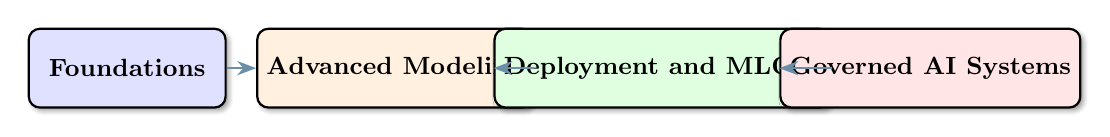
\begin{tikzpicture}[
  box/.style={rectangle, draw, thick, fill=#1, minimum width=2.5cm, minimum height=1.0cm, align=center, font=\small\bfseries, rounded corners=4pt,
    blur shadow={shadow blur steps=4, shadow xshift=0.4mm, shadow yshift=-0.4mm}},
  arr/.style={-{Stealth[length=2.4mm]}, thick, primary!65}
]
  \node[box=blue!12] (f1) at (0,0) {Foundations};
  \node[box=orange!12] (f2) at (3.4,0) {Advanced Modeling};
  \node[box=green!12] (f3) at (6.8,0) {Deployment and MLOps};
  \node[box=red!10] (f4) at (10.2,0) {Governed AI Systems};

  \draw[arr] (f1) -- (f2);
  \draw[arr] (f2) -- (f3);
  \draw[arr] (f3) -- (f4);
\end{tikzpicture}
\end{center}

%=============================================================
\section{Advanced Problem Framing and Project Design}
%=============================================================

\begin{definitionbox}[Problem Framing]
Problem framing is the process of converting a real-world question into a clear analytical or machine learning task with measurable success criteria, known constraints, and a deployment context.
\end{definitionbox}

\subsection{From Real Problem to Data Science Task}

\rowcolors{2}{white}{defbg}
\begin{longtable}{@{}p{4.0cm}p{4.0cm}p{5.0cm}@{}}
\toprule
\rowcolor{primary!15}
\textbf{Real-World Goal} & \textbf{Data Science Formulation} & \textbf{Possible Metrics} \\
\midrule
\endhead
Identify at-risk students & Binary classification & Recall, precision, F1-score, calibration \\
\addlinespace
Forecast course enrollment & Time series forecasting & MAE, RMSE, MAPE \\
\addlinespace
Recommend learning materials & Ranking or recommendation & Precision@k, Recall@k, NDCG \\
\addlinespace
Detect unusual student system behavior & Anomaly detection & Detection rate, false alarm rate \\
\bottomrule
\end{longtable}

\subsection{Advanced Success Criteria}

\begin{itemize}[leftmargin=*]
  \item \textbf{Offline metrics:} Accuracy, RMSE, F1-score, AUC, ranking metrics.
  \item \textbf{Operational metrics:} Latency, throughput, availability, compute cost.
  \item \textbf{Business or institutional metrics:} Retention rate, intervention success, decision quality.
  \item \textbf{Safety and governance metrics:} Bias, drift, privacy compliance, reviewability.
\end{itemize}

\begin{alertbox}[Advanced Projects Fail When the Objective Is Vague]
If the project question, metric, user, or decision context is unclear, even a technically strong model may create little value.
\end{alertbox}

\subsection{Constraints and Tradeoffs}

\begin{conceptbox}[Advanced Tradeoffs]
Real systems rarely optimize only one thing. Data Scientists often need to balance accuracy, interpretability, fairness, latency, privacy, compute cost, and maintainability at the same time.
\end{conceptbox}

%=============================================================
\section{Data Architecture, Engineering, and Quality at Scale}
%=============================================================

\subsection{Why Advanced Data Science Needs Engineering}

\begin{itemize}[leftmargin=*]
  \item Models are only as useful as the systems that feed and support them.
  \item Large projects require reliable data ingestion, transformation, storage, versioning, and access control.
  \item Data pipelines make advanced analytics repeatable and production-ready.
\end{itemize}

\subsection{Common Data System Patterns}

\rowcolors{2}{white}{defbg}
\begin{longtable}{@{}p{3.0cm}p{3.6cm}p{6.4cm}@{}}
\toprule
\rowcolor{primary!15}
\textbf{System} & \textbf{Main Role} & \textbf{Typical Use} \\
\midrule
\endhead
Data warehouse & Structured analytical storage & BI reporting, dashboarding, tabular analytics \\
\addlinespace
Data lake & Raw and flexible storage & Large-scale raw data, mixed formats, historical storage \\
\addlinespace
Lakehouse & Lake flexibility plus warehouse structure & Unified analytics and machine learning workflows \\
\addlinespace
Feature store & Centralized feature management & Consistent train-serving feature definitions \\
\bottomrule
\end{longtable}

\subsection{ETL vs. ELT}

\begin{itemize}[leftmargin=*]
  \item \textbf{ETL:} Extract, transform, then load. Useful when transformation must happen before storage.
  \item \textbf{ELT:} Extract, load, then transform. Common in modern cloud analytics where storage and computation are flexible.
\end{itemize}

\subsection{Batch vs. Streaming}

\begin{center}
\begin{tabular}{@{}p{6.2cm}p{6.2cm}@{}}
\toprule
\textbf{Batch Processing} & \textbf{Streaming Processing} \\
\midrule
Handles data in chunks or scheduled runs & Handles data continuously as events arrive \\
Suitable for daily or hourly pipelines & Suitable for real-time detection and alerting \\
Simpler to manage & Lower latency but more complex engineering \\
\bottomrule
\end{tabular}
\end{center}

\subsection{Data Quality Dimensions}

\rowcolors{2}{white}{defbg}
\begin{longtable}{@{}p{3.0cm}p{10cm}@{}}
\toprule
\rowcolor{primary!15}
\textbf{Dimension} & \textbf{Meaning} \\
\midrule
\endhead
Completeness & Required values are present \\
\addlinespace
Validity & Data matches allowed formats and rules \\
\addlinespace
Consistency & Data agrees across systems and time \\
\addlinespace
Uniqueness & Duplicate records are controlled \\
\addlinespace
Timeliness & Data is fresh enough for the use case \\
\addlinespace
Lineage & The origin and transformation history are traceable \\
\bottomrule
\end{longtable}

\begin{conceptbox}[Data Lineage]
Data lineage means knowing where the data came from, how it was transformed, and which downstream models or dashboards depend on it. This is essential for debugging, trust, and governance.
\end{conceptbox}

\subsection{Advanced Pipeline View}

\begin{center}
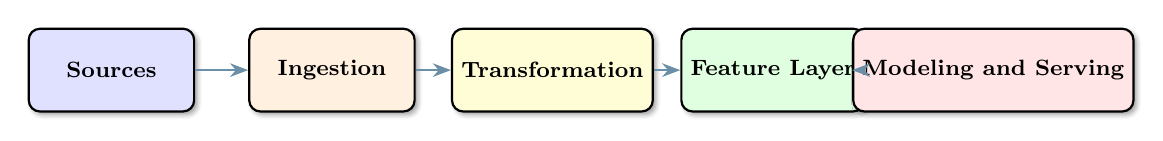
\begin{tikzpicture}[
  step/.style={rectangle, draw, thick, fill=#1, minimum width=2.1cm, minimum height=1.05cm, align=center, font=\footnotesize\bfseries, rounded corners=4pt,
    blur shadow={shadow blur steps=4, shadow xshift=0.4mm, shadow yshift=-0.4mm}},
  arr/.style={-{Stealth[length=2.3mm]}, thick, primary!65}
]
  \node[step=blue!12] (p1) at (0,0) {Sources};
  \node[step=orange!12] (p2) at (2.8,0) {Ingestion};
  \node[step=yellow!16] (p3) at (5.6,0) {Transformation};
  \node[step=green!12] (p4) at (8.4,0) {Feature Layer};
  \node[step=red!10] (p5) at (11.2,0) {Modeling and Serving};

  \draw[arr] (p1) -- (p2);
  \draw[arr] (p2) -- (p3);
  \draw[arr] (p3) -- (p4);
  \draw[arr] (p4) -- (p5);
\end{tikzpicture}
\end{center}

%=============================================================
\section{Advanced Statistical Thinking and Experimental Design}
%=============================================================

\subsection{Why Statistics Still Matters}

\begin{itemize}[leftmargin=*]
  \item Advanced Data Science is not only about bigger models.
  \item Statistical thinking helps us judge whether patterns are real, whether estimates are stable, and whether conclusions can be trusted.
\end{itemize}

\subsection{Key Statistical Ideas for Advanced Practice}

\begin{itemize}[leftmargin=*]
  \item \textbf{Sampling bias:} The collected data does not represent the true population well.
  \item \textbf{Variance:} Model performance may change strongly across different samples.
  \item \textbf{Confidence intervals:} A range of plausible values for an estimate.
  \item \textbf{Hypothesis testing:} A formal way to check whether an observed effect is likely meaningful.
  \item \textbf{Statistical significance vs practical significance:} A small measurable effect may still be too weak to matter in practice.
\end{itemize}

\subsection{Correlation vs. Causation}

\begin{alertbox}[Do Not Confuse Association with Cause]
Two variables can move together without one causing the other. Advanced Data Science often requires asking whether a pattern is merely predictive or actually useful for intervention and decision-making.
\end{alertbox}

\subsection{A/B Testing and Controlled Experiments}

\begin{definitionbox}[A/B Test]
An A/B test compares two versions of a system, intervention, or interface to determine which one performs better on a chosen metric. It is one of the most common methods for measuring causal impact in digital systems.
\end{definitionbox}

\begin{itemize}[leftmargin=*]
  \item Define the treatment and control groups clearly.
  \item Choose one main evaluation metric before running the experiment.
  \item Ensure random assignment when possible.
  \item Consider sample size, duration, and possible confounding factors.
\end{itemize}

%=============================================================
\section{Advanced Feature Engineering and Representation Learning}
%=============================================================

\subsection{Beyond Basic Feature Engineering}

\begin{itemize}[leftmargin=*]
  \item Create interaction features between variables.
  \item Build lag features for time series data.
  \item Use domain-driven aggregates such as weekly averages or activity counts.
  \item Add derived behavioral indicators such as engagement trend or risk score.
\end{itemize}

\subsection{Important Advanced Techniques}

\rowcolors{2}{white}{defbg}
\begin{longtable}{@{}p{3.2cm}p{4.0cm}p{5.8cm}@{}}
\toprule
\rowcolor{primary!15}
\textbf{Technique} & \textbf{Purpose} & \textbf{Notes} \\
\midrule
\endhead
Scaling and normalization & Put variables on comparable ranges & Important for distance-based models and neural networks \\
\addlinespace
Encoding & Represent categorical variables numerically & One-hot, ordinal, target, and embedding-based approaches \\
\addlinespace
Feature selection & Reduce noise and improve interpretability & Filter, wrapper, embedded, or model-based approaches \\
\addlinespace
Dimensionality reduction & Compress information into fewer features & PCA, UMAP, autoencoders \\
\addlinespace
Embeddings & Dense vector representations & Powerful for text, images, users, items, and multimodal tasks \\
\bottomrule
\end{longtable}

\subsection{Representation Learning}

\begin{definitionbox}[Representation Learning]
Representation learning refers to methods that automatically learn useful internal representations of data instead of relying entirely on manual feature creation. Deep learning models are especially strong in this area.
\end{definitionbox}

\begin{conceptbox}[Embeddings in Advanced Data Science]
Embeddings are no longer limited to language models. They are widely used for recommendation, semantic search, similarity analysis, anomaly detection, and multimodal systems.
\end{conceptbox}

\subsection{Data Leakage}

\begin{alertbox}[A Common Advanced Mistake]
Data leakage happens when information that would not be available at prediction time accidentally enters training. Leakage can make a model look excellent during evaluation and fail badly in the real world.
\end{alertbox}

%=============================================================
\section{Advanced Model Families and Learning Strategies}
%=============================================================

\subsection{Ensemble Methods}

\begin{definitionbox}[Ensemble Learning]
Ensemble methods combine multiple models to produce a stronger result than a single model alone. They are often highly competitive on structured tabular data.
\end{definitionbox}

\begin{itemize}[leftmargin=*]
  \item \textbf{Bagging:} Trains models in parallel on varied samples to reduce variance.
  \item \textbf{Boosting:} Trains models sequentially so each new model focuses on earlier errors.
  \item \textbf{Stacking:} Combines multiple model outputs using a meta-model.
\end{itemize}

\subsection{Advanced Supervised Models}

\begin{itemize}[leftmargin=*]
  \item Random Forest and Extra Trees
  \item Gradient Boosting, XGBoost, LightGBM, CatBoost
  \item Support Vector Machines in selected high-dimensional settings
  \item Neural networks for tabular, text, image, and multimodal tasks
\end{itemize}

\subsection{Validation and Generalization}

\begin{itemize}[leftmargin=*]
  \item \textbf{Cross-validation:} Repeatedly evaluate across different folds to estimate stability.
  \item \textbf{Backtesting:} Use time-aware validation for forecasting tasks.
  \item \textbf{Nested validation:} Separate tuning and evaluation more carefully for stronger estimates.
\end{itemize}

\subsection{Hyperparameter Tuning}

\begin{itemize}[leftmargin=*]
  \item Grid search tries all combinations in a chosen grid.
  \item Random search explores many combinations more efficiently in large spaces.
  \item Bayesian optimization uses prior observations to choose promising settings.
\end{itemize}

\subsection{Imbalanced Learning}

\begin{conceptbox}[Imbalanced Data]
In many real datasets, the important class is also the rare class. Fraud cases, dropout events, equipment failures, and serious incidents may be much less frequent than normal cases.
\end{conceptbox}

Useful responses include:
\begin{itemize}[leftmargin=*]
  \item Class weighting
  \item Resampling or synthetic sampling
  \item Threshold tuning
  \item Metrics beyond raw accuracy
\end{itemize}

\subsection{Calibration and Explainability}

\begin{itemize}[leftmargin=*]
  \item \textbf{Calibration:} Makes predicted probabilities better aligned with actual observed frequencies.
  \item \textbf{Global explainability:} Helps understand overall model behavior.
  \item \textbf{Local explainability:} Helps explain one specific prediction.
  \item Common tools include feature importance, SHAP, permutation importance, and partial dependence plots.
\end{itemize}

%=============================================================
\section{Specialized Advanced Problem Settings}
%=============================================================

\subsection{Time Series and Forecasting}

\begin{definitionbox}[Time Series]
Time series data is ordered in time. This creates additional structure such as trend, seasonality, cycles, events, and temporal dependence.
\end{definitionbox}

Key considerations:
\begin{itemize}[leftmargin=*]
  \item Respect time order during validation.
  \item Use lag features and rolling summaries when appropriate.
  \item Check for seasonality and trend.
  \item Monitor forecast decay over time.
\end{itemize}

Common models:
\begin{itemize}[leftmargin=*]
  \item ARIMA-like statistical models
  \item Prophet-like business forecasting models
  \item Gradient boosting with lag features
  \item LSTM and transformer-based forecasting models
\end{itemize}

\subsection{Anomaly Detection}

\begin{definitionbox}[Anomaly Detection]
Anomaly detection identifies unusual observations, patterns, or events that differ significantly from normal behavior.
\end{definitionbox}

Examples:
\begin{itemize}[leftmargin=*]
  \item Unusual login patterns
  \item Suspicious transactions
  \item Sudden equipment failures
  \item Rare academic behavior signals
\end{itemize}

\subsection{Recommendation Systems}

\begin{itemize}[leftmargin=*]
  \item \textbf{Content-based filtering:} Recommends items similar to those already preferred.
  \item \textbf{Collaborative filtering:} Uses patterns from many users and items.
  \item \textbf{Hybrid recommenders:} Combine both approaches.
\end{itemize}

\subsection{Graph and Network Analytics}

\begin{conceptbox}[Graph Data]
Some advanced Data Science problems are best viewed as networks rather than tables. Examples include social networks, citation graphs, communication networks, and linked educational systems.
\end{conceptbox}

%=============================================================
\section{Deep Learning, Foundation Models, and AI-Assisted Workflows}
%=============================================================

\subsection{Deep Learning in Advanced Data Science}

\begin{itemize}[leftmargin=*]
  \item Convolutional Neural Networks for images and spatial patterns
  \item Recurrent and sequence models for temporal or language data
  \item Transformers for language, multimodal systems, and foundation models
  \item Autoencoders and contrastive methods for representation learning
\end{itemize}

\subsection{Transfer Learning and Fine-Tuning}

\begin{definitionbox}[Transfer Learning]
Transfer learning reuses a model trained on a large task and adapts it to a smaller or more specialized task. This is often more practical than training from scratch.
\end{definitionbox}

\begin{definitionbox}[Fine-Tuning]
Fine-tuning means continuing training on a pretrained model using a domain-specific dataset so that the model becomes better suited to a particular application.
\end{definitionbox}

\subsection{Foundation Models in Data Science}

\begin{itemize}[leftmargin=*]
  \item Large Language Models for summarization, question answering, code generation, and semantic search
  \item Vision models for classification, detection, and image understanding
  \item Multimodal models that combine text, image, and audio inputs
\end{itemize}

\subsection{Retrieval-Augmented Generation (RAG)}

\begin{definitionbox}[RAG]
Retrieval-Augmented Generation combines information retrieval with generation. The system first retrieves relevant content from trusted sources, then uses that content to produce a grounded answer.
\end{definitionbox}

\begin{conceptbox}[Why RAG Matters]
RAG is highly relevant in advanced Data Science systems because it improves accuracy, traceability, and domain adaptation without always requiring full fine-tuning.
\end{conceptbox}

\subsection{AI-Assisted Data Science Workflows}

\begin{itemize}[leftmargin=*]
  \item GitHub Copilot can accelerate coding, notebook drafting, and error explanation.
  \item Large language models can help summarize data documentation and generate SQL or Python scaffolds.
  \item Agentic systems can orchestrate analysis, reporting, and validation tasks.
\end{itemize}

\begin{alertbox}[Productivity Does Not Remove Responsibility]
AI coding assistants can help advanced Data Science work, but they do not replace testing, validation, reproducibility, or domain understanding.
\end{alertbox}

%=============================================================
\section{MLOps, Deployment, and Monitoring}
%=============================================================

\begin{definitionbox}[MLOps]
MLOps is the set of practices that brings machine learning systems into reliable production by combining machine learning, software engineering, DevOps, monitoring, and governance.
\end{definitionbox}

\subsection{Core MLOps Capabilities}

\rowcolors{2}{white}{defbg}
\begin{longtable}{@{}p{3.2cm}p{9.8cm}@{}}
\toprule
\rowcolor{primary!15}
\textbf{Capability} & \textbf{Why It Matters} \\
\midrule
\endhead
Experiment tracking & Compare runs, parameters, and results systematically \\
\addlinespace
Model registry & Store approved versions of models for reuse and deployment \\
\addlinespace
Versioning & Track code, data, and model changes consistently \\
\addlinespace
CI/CD for ML & Automate testing and deployment of data and model changes \\
\addlinespace
Monitoring & Detect drift, failures, latency changes, and performance decline \\
\addlinespace
Rollback and retraining & Recover safely and improve models over time \\
\bottomrule
\end{longtable}

\subsection{Deployment Patterns}

\begin{itemize}[leftmargin=*]
  \item \textbf{Batch scoring:} Run predictions on a schedule.
  \item \textbf{Real-time API serving:} Generate predictions on demand.
  \item \textbf{Streaming inference:} Score live events continuously.
  \item \textbf{Edge deployment:} Run models close to the device or sensor.
\end{itemize}

\subsection{Monitoring in Production}

\begin{itemize}[leftmargin=*]
  \item \textbf{Data drift:} Input data distribution changes.
  \item \textbf{Concept drift:} The relationship between inputs and outputs changes.
  \item \textbf{Performance drift:} Quality metrics decline over time.
  \item \textbf{Operational drift:} Latency, uptime, or cost changes unexpectedly.
\end{itemize}

\begin{center}
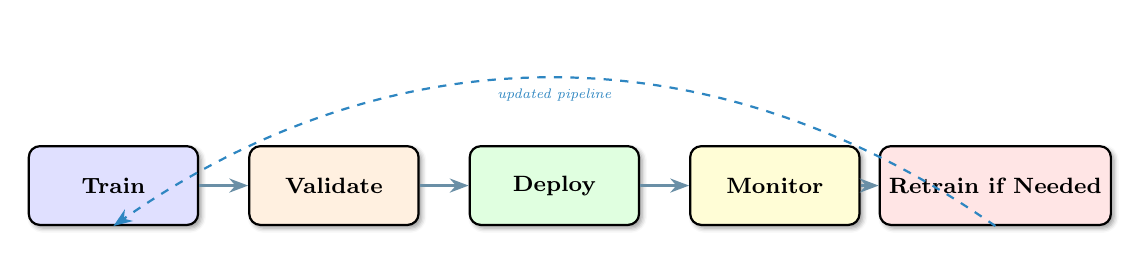
\begin{tikzpicture}[
  step/.style={rectangle, draw, thick, fill=#1, minimum width=2.15cm, minimum height=1.0cm, align=center, font=\footnotesize\bfseries, rounded corners=4pt,
    blur shadow={shadow blur steps=4, shadow xshift=0.4mm, shadow yshift=-0.4mm}},
  arr/.style={-{Stealth[length=2.4mm]}, thick, primary!65}
]
  \node[step=blue!12] (m1) at (0,0) {Train};
  \node[step=orange!12] (m2) at (2.8,0) {Validate};
  \node[step=green!12] (m3) at (5.6,0) {Deploy};
  \node[step=yellow!16] (m4) at (8.4,0) {Monitor};
  \node[step=red!10] (m5) at (11.2,0) {Retrain if Needed};

  \draw[arr] (m1) -- (m2);
  \draw[arr] (m2) -- (m3);
  \draw[arr] (m3) -- (m4);
  \draw[arr] (m4) -- (m5);
  \draw[arr, dashed, secondary] (m5.south) to[bend right=35] node[below, font=\tiny\itshape, secondary] {updated pipeline} (m1.south);
\end{tikzpicture}
\end{center}

\subsection{Reproducibility}

\begin{conceptbox}[Reproducibility]
Reproducibility means that another person, or the same team later, can rerun the pipeline and reach the same result with the same code, data, configuration, and environment.
\end{conceptbox}

\begin{lstlisting}
run = tracker.start_run("xgboost_student_risk")
run.log_params(best_params)
run.log_metrics({"f1": 0.84, "recall": 0.88})
run.register_model(model, name="student-risk-model")
\end{lstlisting}

%=============================================================
\section{Governance, Ethics, and Secure Advanced Practice}
%=============================================================

\subsection{Governance as a Technical Requirement}

\begin{itemize}[leftmargin=*]
  \item Governance is not only policy; it is also system design.
  \item Advanced Data Science systems should be auditable, documented, and reviewable.
  \item Responsible systems define who can access data, approve deployment, and respond to failures.
\end{itemize}

\subsection{Major Governance Themes}

\rowcolors{2}{white}{defbg}
\begin{longtable}{@{}p{3.1cm}p{4.1cm}p{5.8cm}@{}}
\toprule
\rowcolor{primary!15}
\textbf{Theme} & \textbf{Main Concern} & \textbf{Typical Response} \\
\midrule
\endhead
Fairness & Unequal treatment across groups & Bias testing, subgroup analysis, review \\
\addlinespace
Privacy & Exposure of sensitive data & Access control, minimization, anonymization \\
\addlinespace
Security & Unauthorized use or model abuse & Authentication, logging, red teaming \\
\addlinespace
Explainability & Hard-to-understand decisions & Model interpretation and human review \\
\addlinespace
Accountability & Who owns the system and outcomes & Documentation, approval workflows, audit trails \\
\bottomrule
\end{longtable}

\subsection{Useful Documentation Artifacts}

\begin{itemize}[leftmargin=*]
  \item \textbf{Model cards:} High-level summaries of intended use, limitations, and performance.
  \item \textbf{Datasheets for datasets:} Structured documentation about how data was collected and what risks exist.
  \item \textbf{Runbooks:} Practical operating instructions for failures and monitoring alerts.
\end{itemize}

\begin{alertbox}[Advanced Systems Need Human Oversight]
The more autonomous and high-impact a system becomes, the more important human approval, monitoring, and escalation paths become.
\end{alertbox}

%=============================================================
\section{BSIT Case Study: Student Success and Academic Risk Platform}
%=============================================================

\begin{definitionbox}[Scenario]
A BSIT department wants to build an advanced platform that predicts student risk, recommends interventions, monitors system behavior, and provides dashboards for advisers and instructors.
\end{definitionbox}

\subsection{Possible End-to-End Design}

\begin{enumerate}[leftmargin=*]
  \item Collect data from the LMS, attendance system, grade book, and advising records.
  \item Build an ingestion and transformation pipeline into a curated analytical layer.
  \item Engineer features such as attendance trend, assignment lateness, quiz volatility, and support history.
  \item Compare baseline models with gradient boosting and neural approaches.
  \item Calibrate probabilities so intervention thresholds are meaningful.
  \item Deploy a scoring service and adviser dashboard.
  \item Monitor drift, performance decline, and subgroup fairness.
  \item Retrain periodically as new cohorts and policies change.
\end{enumerate}

\subsection{Why This Is an Advanced Data Science Problem}

\begin{itemize}[leftmargin=*]
  \item It combines tabular data, time trends, deployment, and governance.
  \item It requires both predictive accuracy and responsible institutional use.
  \item It needs monitoring because student behavior and academic policies evolve.
\end{itemize}

\begin{alertbox}[Educational Use Principle]
Such a system should support advisers and teachers, not replace human judgment. Predictions can inform intervention, but they should not act as automatic final decisions.
\end{alertbox}

%=============================================================
\section{Key Takeaways}
%=============================================================

\begin{itemize}[leftmargin=*]
  \item Advanced Data Science extends the beginner lifecycle into engineering, deployment, monitoring, and governance.
  \item Strong systems depend on both advanced models and high-quality data architecture.
  \item Statistical thinking remains essential for evaluation, experimentation, and trust.
  \item Feature engineering, representation learning, and validation strategy often matter as much as model choice.
  \item Modern advanced work includes ensembles, deep learning, foundation models, and AI-assisted workflows.
  \item MLOps is necessary for turning models into reliable real systems.
  \item Ethics, privacy, explainability, and accountability are central to advanced professional practice.
\end{itemize}

%=============================================================
\section{Review Questions}
%=============================================================

\begin{enumerate}[leftmargin=*]
  \item What makes Advanced Data Science different from foundational Data Science?
  \item Why is problem framing critical before model building begins?
  \item What is the difference between a data warehouse, data lake, and lakehouse?
  \item Why do advanced systems care about data lineage and feature consistency?
  \item Why is statistical significance not the same as practical usefulness?
  \item What is data leakage, and why is it dangerous?
  \item How do bagging, boosting, and stacking differ?
  \item Why must forecasting tasks use time-aware validation instead of random splitting?
  \item What is the role of transfer learning and fine-tuning in modern AI systems?
  \item What are the core responsibilities of MLOps?
  \item What kinds of drift should be monitored after deployment?
  \item Why are fairness, privacy, explainability, and accountability essential in advanced Data Science?
\end{enumerate}

\end{document}